\documentclass{article}

\usepackage[fontsize=13pt]{scrextend}
\usepackage{geometry}
\usepackage{multicol}
\usepackage{lmodern} % For scalable Computer Modern fonts % Ensures proper font encoding
\usepackage{color}
\usepackage{helvet}  % For changing fonts

\usepackage{soul}  % For highlighting

\geometry{
  a4paper,
  left=25mm,
  right=25mm,
  top=25mm,
  bottom=25mm,
  heightrounded,
}



\usepackage{lastpage} % Required to determine the last page number for the footer

\usepackage{graphicx} % Required to insert images

\setlength\parindent{0pt} % Removes all indentation from paragraphs

\usepackage[most]{tcolorbox} % Required for boxes that split across pages

\usepackage{booktabs} % Required for better horizontal rules in tables

\usepackage{listings} % Required for insertion of code

\usepackage{etoolbox} % Required for if statements

%----------------------------------------------------------------------------------------
%	MARGINS
%----------------------------------------------------------------------------------------

\usepackage{geometry} % Required for adjusting page dimensions and margins

\geometry{
	paper=a4paper, % Change to letterpaper for US letter
	top=3cm, % Top margin
	bottom=3cm, % Bottom margin
	left=2.5cm, % Left margin
	right=2.5cm, % Right margin
	headheight=14pt, % Header height
	footskip=1.4cm, % Space from the bottom margin to the baseline of the footer
	headsep=1.2cm, % Space from the top margin to the baseline of the header
	%showframe, % Uncomment to show how the type block is set on the page
}

%----------------------------------------------------------------------------------------
%	FONT
%----------------------------------------------------------------------------------------

\usepackage[utf8]{inputenc} % Required for inputting international characters
\usepackage[T1]{fontenc} % Output font encoding for international characters

\usepackage[sfdefault,light]{roboto} % Use the Roboto font

%----------------------------------------------------------------------------------------
%	HEADERS AND FOOTERS
%----------------------------------------------------------------------------------------

\usepackage{fancyhdr} % Required for customising headers and footers

\pagestyle{fancy} % Enable custom headers and footers

\lhead{\small\assignmentClass\ifdef{\assignmentClassInstructor}{\ (\assignmentClassInstructor):}{}\ \assignmentTitle} % Left header; output the instructor in brackets if one was set
\chead{} % Centre header
\rhead{\small\ifdef{\assignmentAuthorName}{\assignmentAuthorName}{\ifdef{\assignmentDueDate}{Due\ \assignmentDueDate}{}}} % Right header; output the author name if one was set, otherwise the due date if that was set

\lfoot{} % Left footer
\cfoot{\small Page\ \thepage\ of\ \pageref{LastPage}} % Centre footer
\rfoot{} % Right footer

\renewcommand\headrulewidth{0.5pt} % Thickness of the header rule

%----------------------------------------------------------------------------------------
%	MODIFY SECTION STYLES
%----------------------------------------------------------------------------------------

\usepackage{titlesec} % Required for modifying sections
\usepackage{longtable}
%------------------------------------------------
% Section

\titleformat
{\section} % Section type being modified
[block] % Shape type, can be: hang, block, display, runin, leftmargin, rightmargin, drop, wrap, frame
{\Large\bfseries} % Format of the whole section
{\assignmentQuestionName~\thesection} % Format of the section label
{6pt} % Space between the title and label
{} % Code before the label

\titlespacing{\section}{0pt}{0.5\baselineskip}{0.5\baselineskip} % Spacing around section titles, the order is: left, before and after

%------------------------------------------------
% Subsection

\titleformat
{\subsection} % Section type being modified
[block] % Shape type, can be: hang, block, display, runin, leftmargin, rightmargin, drop, wrap, frame
{\itshape} % Format of the whole section
{(\alph{subsection})} % Format of the section label
{4pt} % Space between the title and label
{} % Code before the label

\titlespacing{\subsection}{0pt}{0.5\baselineskip}{0.5\baselineskip} % Spacing around section titles, the order is: left, before and after

\renewcommand\thesubsection{(\alph{subsection})}

%----------------------------------------------------------------------------------------
%	CUSTOM QUESTION COMMANDS/ENVIRONMENTS
%----------------------------------------------------------------------------------------

% Environment to be used for each question in the assignment
\newenvironment{question}{
	\vspace{0.5\baselineskip} % Whitespace before the question
	\section{} % Blank section title (e.g. just Question 2)
	\lfoot{\small\itshape\assignmentQuestionName~\thesection~continued on next page\ldots} % Set the left footer to state the question continues on the next page, this is reset to nothing if it doesn't (below)
}{
	\lfoot{} % Reset the left footer to nothing if the current question does not continue on the next page
}

%------------------------------------------------

% Environment for subquestions, takes 1 argument - the name of the section
\newenvironment{subquestion}[1]{
	\subsection{#1}
}{
}

%------------------------------------------------

% Command to print a question sentence
\newcommand{\questiontext}[1]{
	\textbf{#1}
	\vspace{0.5\baselineskip} % Whitespace afterwards
}

%------------------------------------------------

% Command to print a box that breaks across pages with the question answer
\newcommand{\answer}[1]{
	\begin{tcolorbox}[breakable, enhanced]
		#1
	\end{tcolorbox}
}

%------------------------------------------------

% Command to print a box that breaks across pages with the space for a student to answer
\newcommand{\answerbox}[1]{
	\begin{tcolorbox}[breakable, enhanced]
		\vphantom{L}\vspace{\numexpr #1-1\relax\baselineskip} % \vphantom{L} to provide a typesetting strut with a height for the line, \numexpr to subtract user input by 1 to make it 0-based as this command is
	\end{tcolorbox}
}

%------------------------------------------------

% Command to print an assignment section title to split an assignment into major parts
\newcommand{\assignmentSection}[1]{
	{
		\centering % Centre the section title
		\vspace{2\baselineskip} % Whitespace before the entire section title
		
		\rule{0.8\textwidth}{0.5pt} % Horizontal rule
		
		\vspace{0.75\baselineskip} % Whitespace before the section title
		{\LARGE \MakeUppercase{#1}} % Section title, forced to be uppercase
		
		\rule{0.8\textwidth}{0.5pt} % Horizontal rule
		
		\vspace{\baselineskip} % Whitespace after the entire section title
	}
}

%----------------------------------------------------------------------------------------
%	TITLE PAGE
%----------------------------------------------------------------------------------------

\author{\textbf{\assignmentAuthorName}} % Set the default title page author field
\date{} % Don't use the default title page date field

\title{
	\thispagestyle{empty} % Suppress headers and footers
	\vspace{0.2\textheight} % Whitespace before the title
	\textbf{\assignmentClass:\ \assignmentTitle}\\[-4pt]
	\ifdef{\assignmentDueDate}{{\small Due\ on\ \assignmentDueDate}\\}{} % If a due date is supplied, output it
	\ifdef{\assignmentClassInstructor}{{\large \textit{\assignmentClassInstructor}}}{} % If an instructor is supplied, output it
	\vspace{0.32\textheight} % Whitespace before the author name
}

\usepackage[utf8]{inputenc}
\usepackage[T1]{fontenc}
\usepackage{lmodern}
\usepackage{booktabs}
\usepackage{xcolor}
\usepackage{tikz}
\usepackage{pgfplots}
\usepackage{graphicx}

\usepackage{amsmath}


\usepackage{amsfonts}
\usepackage{amssymb}

\usepackage{tabularx}



\usepackage{hyperref}
\usepackage{listings}
\usepackage{booktabs}
\usepackage{tabularray}
\usepackage{multirow}
\usepackage{float}
\usepackage{lastpage}
\usepackage{tcolorbox}
\usepackage{titlesec}

\usepackage{etoolbox}

\makeatletter
\patchcmd{\@zfancyhead}{\fancy@reset}{\f@nch@reset}{}{}
\patchcmd{\@set@em@up}{\f@ncyolh}{\f@nch@olh}{}{}
\patchcmd{\@set@em@up}{\f@ncyolh}{\f@nch@olh}{}{}
\patchcmd{\@set@em@up}{\f@ncyorh}{\f@nch@orh}{}{}
\makeatother

\pgfplotsset{compat=newest}

% Colors from structure.tex
\definecolor{secondaryColor}{RGB}{0,0,0}
\definecolor{accentColor1}{RGB}{255,87,34}
\definecolor{accentColor3}{RGB}{63,81,181}
\definecolor{textColor}{RGB}{33,33,33}
\definecolor{primaryColor}{RGB}{34, 45, 101}
\definecolor{accentColor2}{RGB}{46, 117, 182}
\definecolor{backgroundColor}{RGB}{245, 245, 245}
\definecolor{fitcolor}{RGB}{0,128,0}
\definecolor{okaycolor}{RGB}{255,165,0}
\definecolor{notfitcolor}{RGB}{255,0,0}



\definecolor{sectioncolor}{RGB}{0,0,100}  % Deep blue for main headings
\definecolor{subcolor}{RGB}{100,0,100}  % Purple for subheadings
\definecolor{lightRed}{RGB}{255,200,200}  % Light red for section underline
\definecolor{lightPink}{RGB}{255,220,220}  % Light pink for subsection underline


\newcommand{\highlight}[1]{\textsf{\textbf{#1}}}  % For highlighting key terms in sans-serif bold
% Custom underline command
\newcommand{\customunderline}[2]{%
  \par\noindent\rule{0pt}{2ex}\vspace{-0.5in} % Adjust the space here
  \colorbox{#1}{\makebox[\linewidth]{#2}}\par
}

% Section format
\titleformat{\section}
  {\color{sectioncolor}\Huge\bfseries\sffamily}  % Sans-serif, huge, bold, blue
  {}
  {0pt}
  {}
  
 

% Subsection format
\titleformat{\subsection}
  {\color{subcolor}\Large\bfseries\sffamily}  % Sans-serif, large, bold, purple
  {}
  {0pt}
  {}

% % Adjust spacing
% \titlespacing*{\section}{0pt}{3.5ex plus 1ex minus .2ex}{2.3ex plus .2ex}
% \titlespacing*{\subsection}{0pt}{3.25ex plus 1ex minus .2ex}{1.5ex plus .2ex}


% % Modify the question environment to include color
% \renewenvironment{question}{
%   \vspace{0.5\baselineskip}
%   \section{}
%   \lfoot{\small\itshape\color{primaryColor}\assignmentQuestionName~\thesection~continued on next page\ldots}
% }{
%   \lfoot{}
% }

% Modify the answer command to include color
\renewcommand{\answer}[1]{
  \begin{tcolorbox}[
    breakable,
    enhanced,
    colback=backgroundColor,
    colframe=primaryColor,
    coltitle=white,
    title=Answer
  ]
    #1
  \end{tcolorbox}
}

% Modify the assignmentSection command to include color
\renewcommand{\assignmentSection}[1]{
  {
    \centering
    \vspace{2\baselineskip}
    
    \color{primaryColor}\rule{0.8\textwidth}{0.5pt}
    
    \vspace{0.75\baselineskip}
    {\LARGE\color{primaryColor}\MakeUppercase{#1}}
    
    \color{primaryColor}\rule{0.8\textwidth}{0.5pt}
    
    \vspace{\baselineskip}
  }
}

% Modify headers and footers to include color
\lhead{\small\color{primaryColor}\assignmentClass\ifdef{\assignmentClassInstructor}{\ (\assignmentClassInstructor):}{Ayush Kumar Mishra}\ \assignmentTitle}
\rhead{\small\color{secondaryColor}\ifdef{\assignmentAuthorName}{\assignmentAuthorName}{\ifdef{\assignmentDueDate}{Due\ \assignmentDueDate}{}}}
\cfoot{\small\color{primaryColor}Page\ \thepage\ of\ \pageref{LastPage}}

\renewcommand\headrulewidth{0.5pt}
\renewcommand{\headrule}{\hbox to\headwidth{\color{primaryColor}\leaders\hrule height \headrulewidth\hfill}}

\hypersetup{
    colorlinks=true,
    linkcolor=primaryColor,
    filecolor=accentColor1,      
    urlcolor=accentColor3,
    pdftitle={comprehensive Data Analysis on Sale Data},
    pdfpagemode=FullScreen,
}

\title{\textcolor{primaryColor}{\Huge\textbf{Comprehensive Data Analysis on Sale Data}}}
\author{\textcolor{secondaryColor}{\Large Ayush Kumar Mishra}}
\date{\textcolor{secondaryColor}{\today}}

\begin{document}

\maketitle

\newpage
\section*{Dashboard}
  \begin{center}
        \color{red}\rule{1\linewidth}{1mm}
    \end{center}
\begin{center}
\vspace{2in}
    {\Huge  For seeing all the code live interactively, \\
    \vspace{2in}
    Visit  \href{https://ayusheda-assign.streamlit.app/}{Dashboard}}\\
    
    \vspace{0.7in}
   \textbf{ \href{https://ayusheda-assign.streamlit.app/}{https://ayusheda-assign.streamlit.app/}}
\end{center}

\newpage
\tableofcontents

\newpage
\section{1. Introduction}
  \begin{center}
        \color{red}\rule{1\linewidth}{1mm}
    \end{center}
In this document, I will formulate how i did analysis on the data.\\
The data contains information about the orders, customers, products, and sales.\\
The goal of this analysis is to provide insights into customer behavior, sales trends, SKU performance, and other key metrics.\\
The analysis will be performed using Python and various data analysis libraries such as pandas, NumPy, and Matplotlib.
The analysis will cover the following key areas:
\begin{itemize}
    \item Customer behavior analysis
    \item Sales trends analysis
    \item SKU performance analysis
    \item Order analysis
    \item Cohort analysis
    \item Geographic analysis
    \item Time-based analysis
    \item Customer lifetime value (CLV) analysis    
    \item Basket analysis
    \item Price sensitivity analysis
    \item And more...
\end{itemize}

\section{1. Data Preparation and Overview}
\begin{center}
    \color{red}\rule{1\linewidth}{1mm}
\end{center}
    \subsection{Loading and Inspecting the Dataset}
    \begin{center}
        \color{green}\rule{1\linewidth}{0.7mm}
    \end{center}
    \begin{itemize}
        \item Load the dataset and check its structure.{
            \begin{center}
                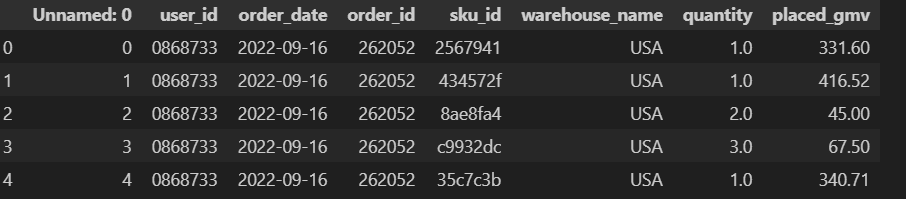
\includegraphics[width=1\columnwidth]{images/data_overview.png}
            \end{center}
            \answer{
                As clearly seen in the image, the dataset contains the following columns:
                \begin{itemize}
                    \item \texttt{Order\_ID}: Unique identifier for each order.
                    \item \texttt{User\_ID}: Unique identifier for each user.
                    \item \texttt{Order\_Date}: Date of the order.
                    \item \texttt{SKU\_ID}: Unique identifier for each product.
                    \item \texttt{Quantity}: Number of items purchased.
                    \item \texttt{Placed\_GMV}: Gross merchandise value (GMV) of the order.
            }
        }
        \item Inspect data for missing values, duplicates, and correct data types.{
            - Their are no missing values and duplicates in the dataset.\\
            \begin{center}
                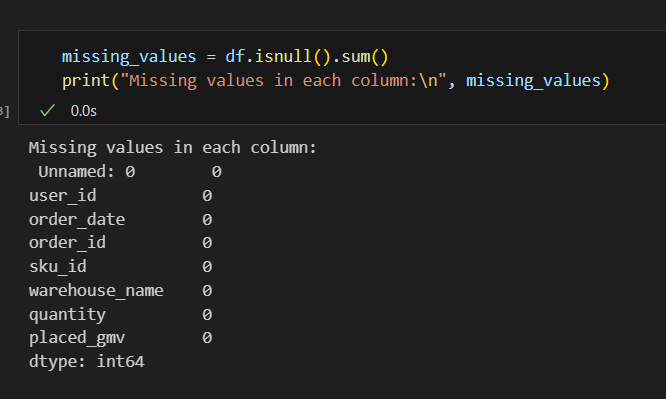
\includegraphics[width=1\columnwidth]{images/missing_values.png}
            \end{center}
        }
    \end{itemize}
    
    \subsection{Statistical Summary}
    \begin{center}
        \color{green}\rule{1\linewidth}{0.7mm}
    \end{center}
    \begin{center}
        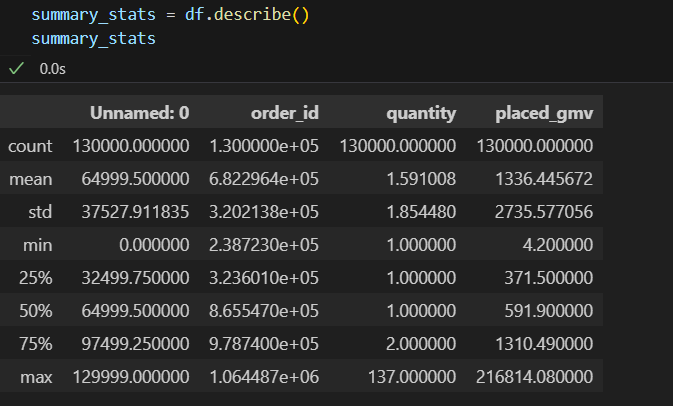
\includegraphics[width=1\columnwidth]{images/data-summary.png}
    \end{center}
    \answer{
       One thing we can observe from summary is that Quantity and Placed GMV are skewed and have outliers.\\
       As 75 percentile is 2 and 50 percentile is 1 for Quantity and 75 percentile is 1310.49 and 50 percentile is 591.90\\
        for Placed GMV.\\
       Whereas their Max values are 137 and 216814 which is much higher than 75 percentile.\\
    }
    
    \subsection{Date Formatting}
    \begin{center}
        \color{green}\rule{1\linewidth}{0.7mm}
    \end{center}
    This step is essential because the date column is in string format. We need to convert it to a datetime format for further analysis.{
        \begin{center}
            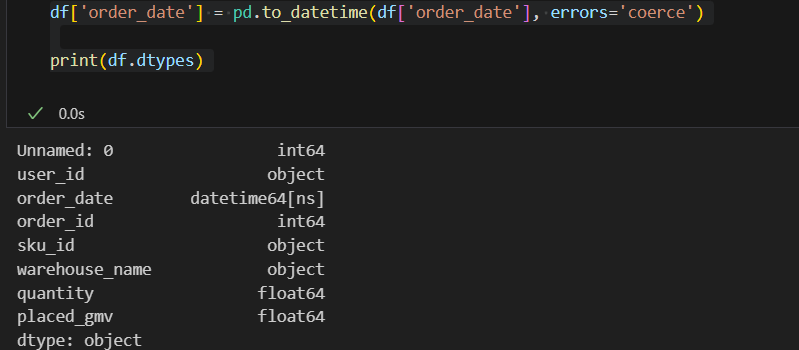
\includegraphics[width=1\columnwidth]{images/datatype.png}
        \end{center}
    }



\section{2. Customer Behavior Analysis}
    \subsection{Customer Purchase Frequency}
    Let's look at the distribution of frequency by which customers are placing orders .{
        \begin{center}
            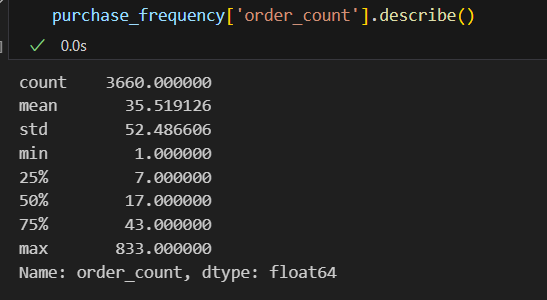
\includegraphics[width=1\columnwidth]{images/order-count.png}
        \end{center}
        \begin{tcolorbox}[colback=lightRed!5!white,colframe=lightRed!75!black,title=Insights]
            \textbf{Insights:}
            \begin{itemize}
                \item More than 50\% of customers have placed orders less than 17 times which is almost half than means\\.
                meaning few people are buying a lot.
                \item And 75\% of customers have placed orders less than 43 times.
                \item Just \textbf{293 people} out of 130000 have placed orders more than 100 times.
            \end{itemize}
        \end{tcolorbox}
    }
    \subsection{Top Customers}
    \begin{itemize}
        \item Based on Order frequency, I am identifying the top customers.{
            \begin{center}
                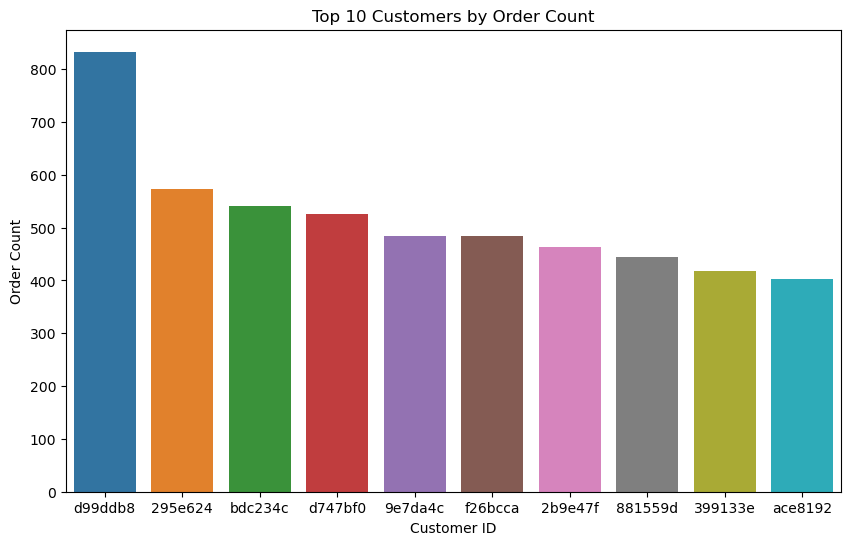
\includegraphics[width=1\columnwidth]{images/customer_purchase_frequency.png}
            \end{center}
        }
        
        
        \item Based on GMV, I am identifying the top customers.{
            \begin{center}
                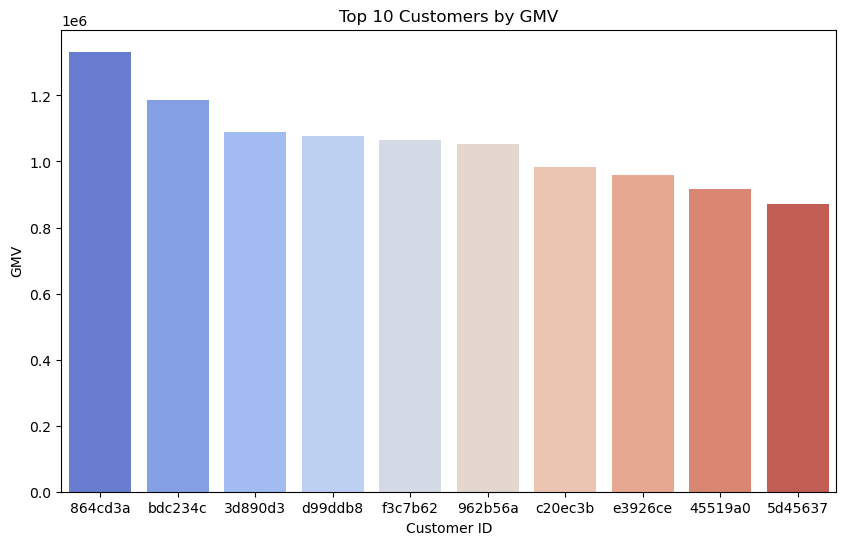
\includegraphics[width=1\columnwidth]{images/top_customers_by_gm.png}
            \end{center}
        }
    \end{itemize}
    
    \subsection{RFM Analysis}
    RFM analysis is a powerful way to segment customers based on their behavior.\\
\begin{itemize}
    \item Recency: When the customer last made a purchase.{
        Here i am calculating the recency of the customers.\\
        \begin{center}
            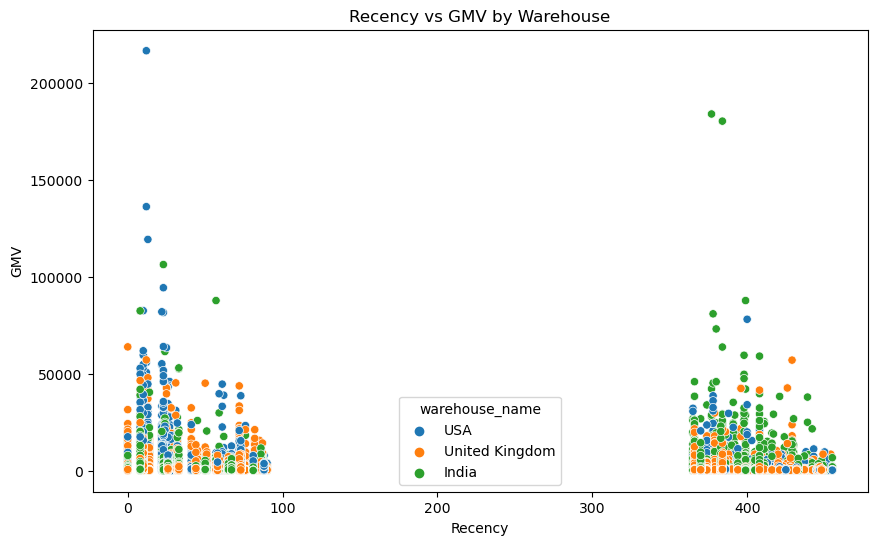
\includegraphics[width=1\columnwidth]{images/recency.png}
        \end{center}
        % use diff color for tcbox everytime
        \begin{tcolorbox}[colback=lightPink!5!white,colframe=lightPink!75!black,title=Insights]
            From the above graph, There are two types of custumers:-
            \begin{itemize}
                \item One who are frequent buyers and have bought recently less than 100 days.
                \item One who are seasonal buyers and have come to buy only after a year.
            \end{itemize}
        \end{tcolorbox}
    }
    \item Frequency: How often the customer made purchases.{
        Here i am calculating the how frequent customers have come to place orders.\\
        \begin{center}
            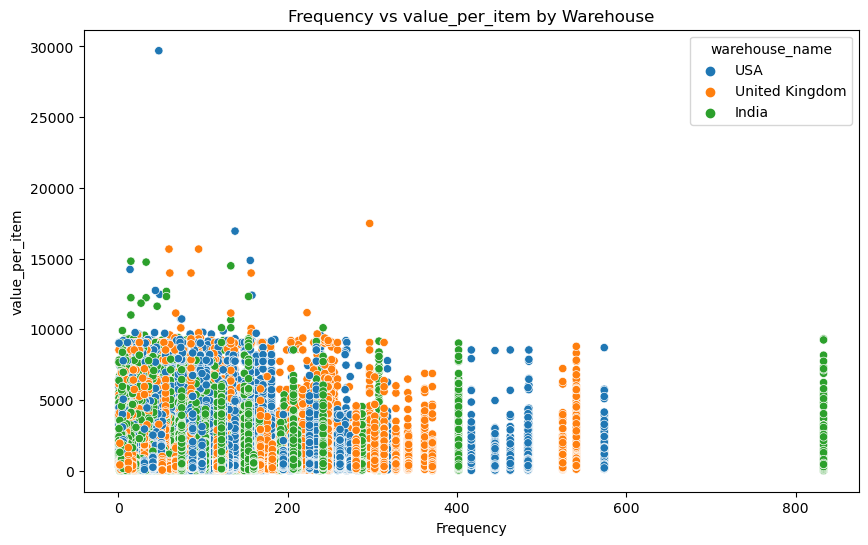
\includegraphics[width=1\columnwidth]{images/Freq_value.png}
        \end{center}
        \begin{tcolorbox}[colback=lightPink!5!white,colframe=lightPink!75!black,title=Insights]
            From the above graph, One observations is that low frequent buyers have more value\_per\_item than high frequent buyers.
        \end{tcolorbox}
    }
    \item Monetary: How much money the customer has spent.{
        Here i am calculating the how much money customers have spent.\\
        \begin{center}
            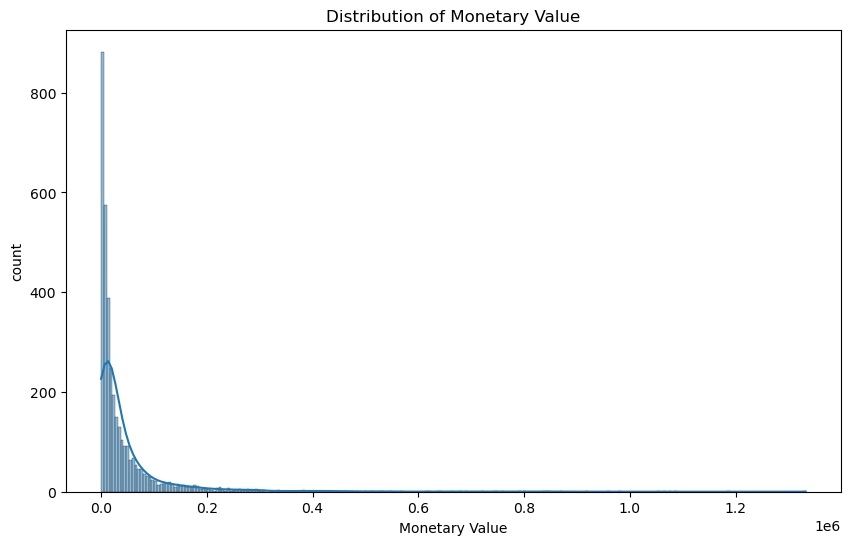
\includegraphics[width=1\columnwidth]{images/dist-mo.png}
        \end{center}
        \begin{tcolorbox}[colback=Pink!5!white,colframe=Pink!75!black,title=Insights]
           Majority of the people have spend less than 0.2 * 10^6.\\
        \end{tcolorbox}
    }
\end{itemize}

Now let's see the relationship between recency, frequency, and monetary values.{
    \begin{center}
        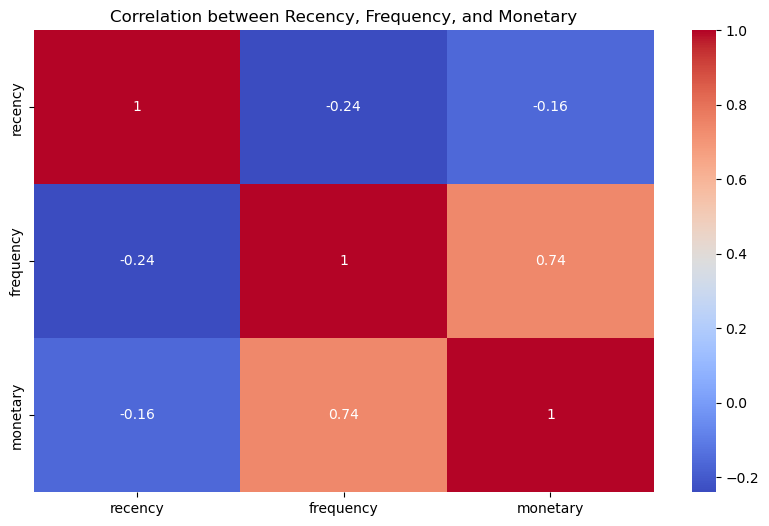
\includegraphics[width=1\columnwidth]{images/rfm.png}
    \end{center}
    \begin{tcolorbox}[colback=backgroundColor, colframe=accentColor2, title=Insights, fonttitle=\bfseries]
        \begin{itemize}
           \item From the above graph, we can see that there is a positive correlation between frequency and monetary value.\\
           \item But there is a negative correlation between recency and frequency and monetary value.\\
        \end{itemize}
       \end{tcolorbox}
}

\large
Score based on all three recency, frequency, and monetary values.\\
\begin{center}
    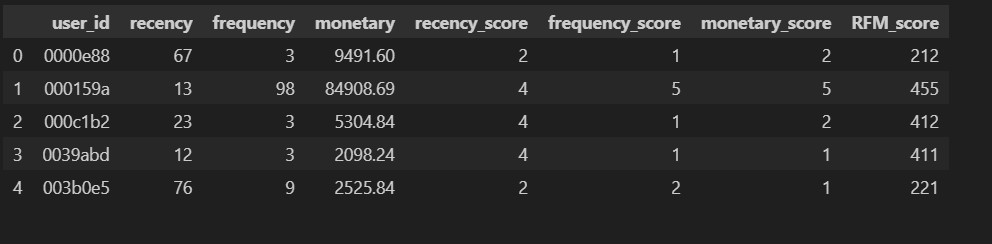
\includegraphics[width=1\columnwidth]{images/rfm-score.png}
\end{center}

\answer{
    Based on this score, i segmented customers into different categories such as:
    \begin{center}
        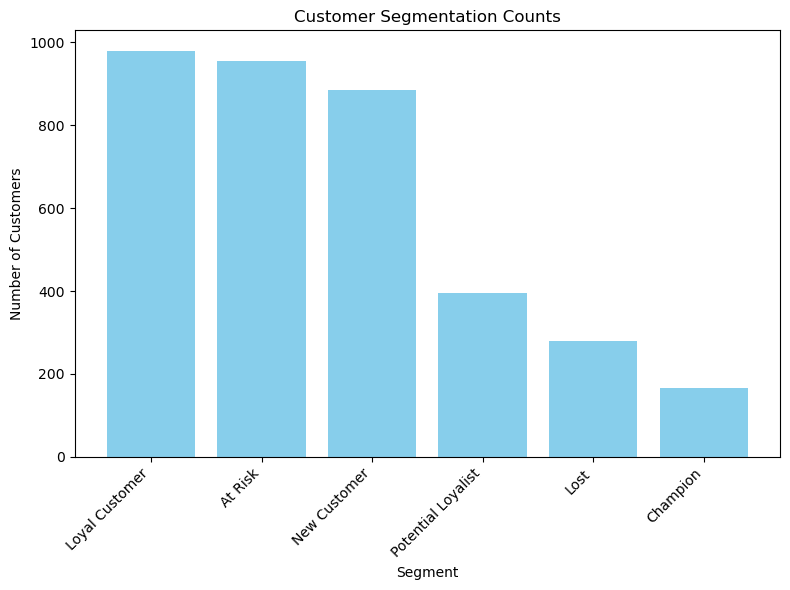
\includegraphics[width=1\columnwidth]{images/custumer-seg.png}
    \end{center}
    \begin{itemize}
        \item \textbf{Champions:} Customers with high recency, frequency, and monetary scores (R = 4-5, F = 4-5, M = 4-5).
        \item \textbf{Loyal Customers:}  Customers with high frequency and monetary scores but may have slightly lower recency (R = 3-5, F = 4-5, M = 4-5).
        \item \textbf{Potential Loyalists:} Customers with high recency and frequency but lower monetary value (R = 4-5, F = 3-5, M = 2-3).
        \item \textbf{New Customers:} High recency.
        \item \textbf{At Risk:} Low recency, frequency, and monetary value.
        \item \textbf{Lost:} Low recency, frequency, and monetary value.
    \end{itemize}
}

    
    
    \subsection{Customer Retention and Churn}
    \begin{itemize}
        \item Analyze customer retention rates and identify potential churn risks.
    \end{itemize}
    \begin{tcolorbox}[colback=blue!5!white, colframe=green!70!black, title= Customer Retention and Churn Rate , fonttitle=\bfseries\Large]
        \begin{center}
            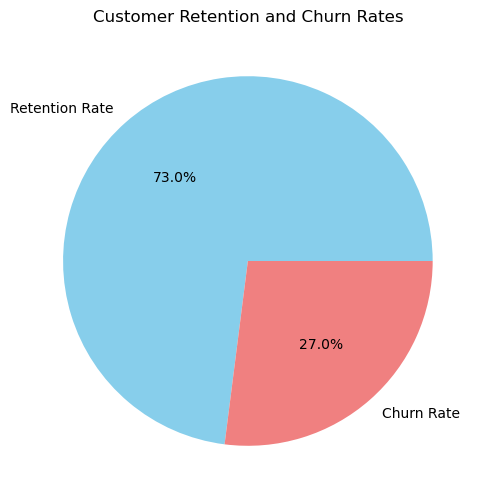
\includegraphics[width=1\columnwidth]{images/crc.png}
        \end{center}
        Clearly from the pie chart we can see that 73\% of the customers are retained and 23\% are churned.\\
    \end{tcolorbox}

\section{3. Sales Trends Analysis}
    \subsection{Time-based Trends}
    \begin{itemize}
        \item Analyze daily, weekly, and monthly sales trends.
    \end{itemize}
   
        \begin{center}
        
        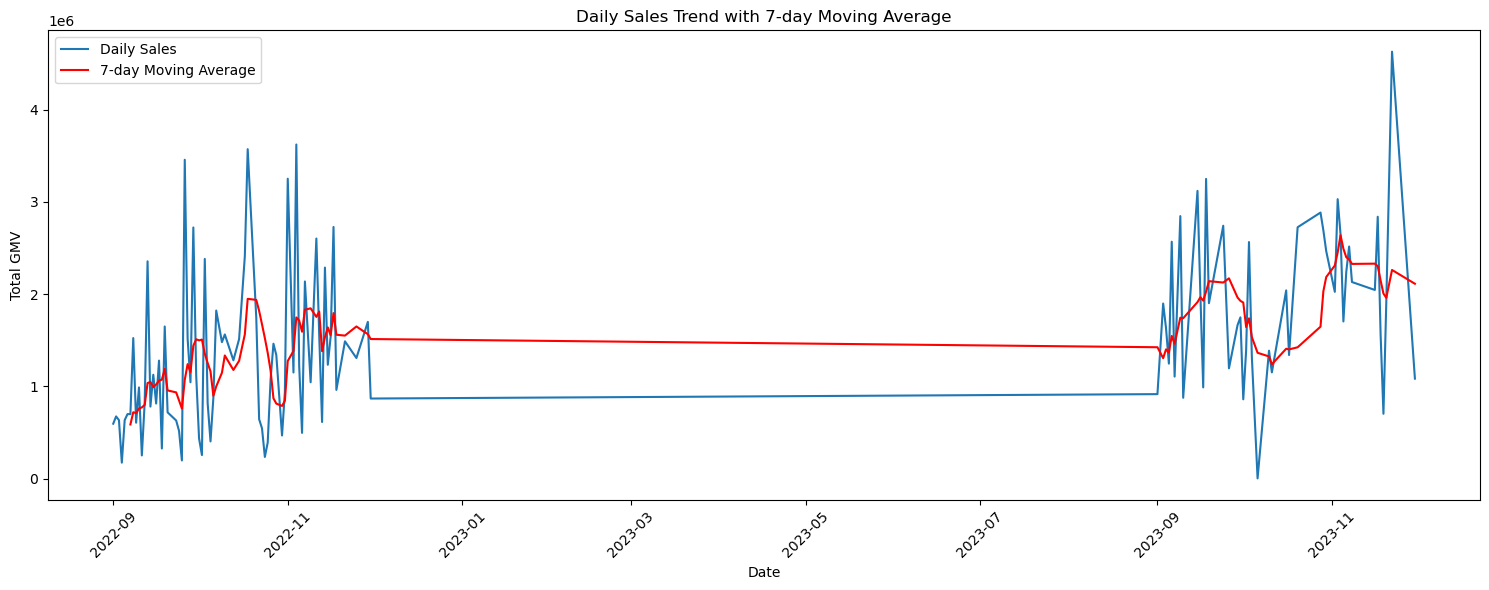
\includegraphics[width=\textwidth]{images/daily.png}
        \caption{Daily sales trends with 7-days moving average.}
    \end{center}
    \begin{center}
        
        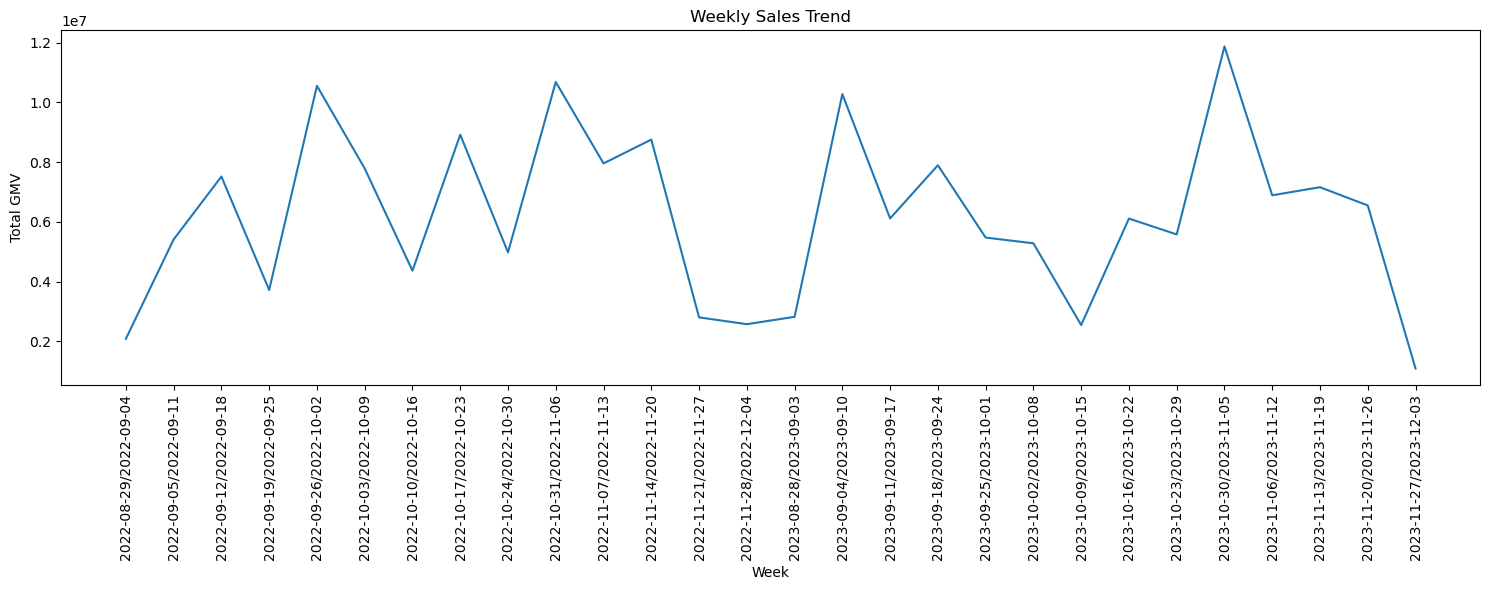
\includegraphics[width=\textwidth]{images/weekly.png}
        \caption{Weekly sales trends.}
    \end{center}
    \begin{center}
        
        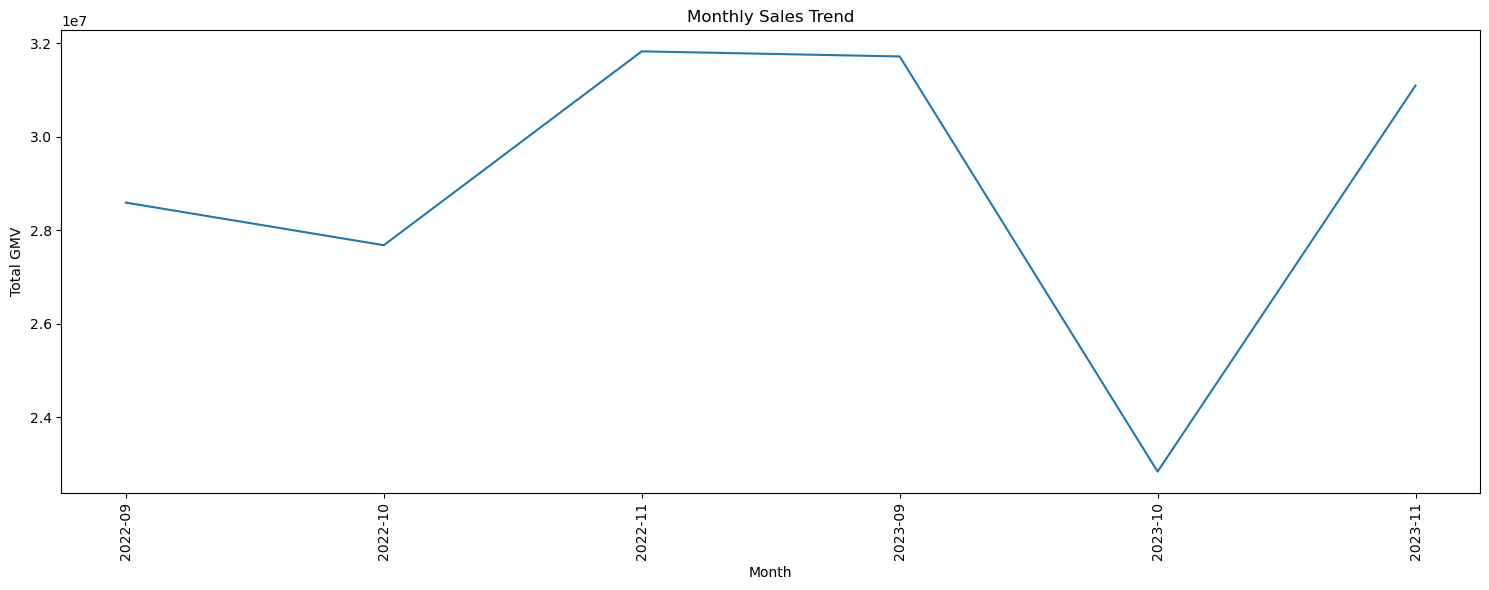
\includegraphics[width=\textwidth]{images/monthly.png}
        \caption{Monthly sales trends.}
    \end{center}
    \caption{Time-based sales trends.}


\subsection{Peak Sales Periods}
\textbf{Identify peak sales periods and any seasonality trends.}
\begin{tcolorbox}[colback=purple!5!white, colframe=purple!75!black, fonttitle=\bfseries, title=Peak Sales Periods by Days]
    \centering
    \begin{tabular}{|c|c|}
    \hline
    \textbf{Order Date} & \textbf{Placed GMV} \\ \hline
    2023-11-22 & 4,629,566.36 \\ \hline 
    2022-11-04 & 3,623,119.11 \\ \hline 
    2022-10-18 & 3,572,387.45 \\ \hline   
    2022-09-26 & 3,457,606.77 \\ \hline 
    2022-11-01 & 3,252,048.05 \\ \hline  
    2023-09-18 & 3,250,288.29 \\ \hline 
    2023-09-15 & 3,120,405.10 \\ \hline 
    2023-11-03 & 3,030,412.93 \\ \hline 
    2023-10-28 & 2,885,263.97 \\ \hline 
    2023-09-09 & 2,846,904.68 \\ \hline 
    \end{tabular}
    \captionof{Top 10 Peak Sales Days}
\end{tcolorbox}
\begin{tcolorbox}[colback=green!5!white, colframe=green!75!black, fonttitle=\bfseries, title=Peak Sales Periods by weeks and months]

    \vspace{0.5cm}

    \centering
    \begin{tabular}{|c|c|}
    \hline
    \textbf{Week} & \textbf{Placed GMV} \\ \hline
    2023-10-30/2023-11-05 & 11,877,473.08 \\ \hline
    2022-10-31/2022-11-06 & 10,685,698.73 \\ \hline
    2022-09-26/2022-10-02 & 10,557,566.61 \\ \hline
    2023-09-04/2023-09-10 & 10,280,051.70 \\ \hline
    2022-10-17/2022-10-23 & 8,919,020.51 \\ \hline
    2022-11-14/2022-11-20 & 8,756,086.30 \\ \hline
    2022-11-07/2022-11-13 & 7,956,940.37 \\ \hline
    2023-09-18/2023-09-24 & 7,895,670.74 \\ \hline
    2022-10-03/2022-10-09 & 7,787,362.60 \\ \hline
    2022-09-12/2022-09-18 & 7,517,063.73 \\ \hline
    \end{tabular}
    \captionof{Top 10 Peak Sales Weeks}

    \vspace{0.5cm}

    \centering
    \begin{tabular}{|c|c|}
    \hline
    \textbf{Month} & \textbf{Placed GMV} \\ \hline
    2022-11 & 31,826,184.02 \\ \hline
    2023-09 & 31,717,114.58 \\ \hline
    2023-11 & 31,094,024.46 \\ \hline
    2022-09 & 28,588,980.49 \\ \hline
    2022-10 & 27,677,926.44 \\ \hline
    2023-10 & 22,833,707.32 \\ \hline
    \end{tabular}
    \captionof{Top 10 Peak Sales Months}

    \vspace{0.5cm}

\end{tcolorbox}


\textbf{From above tables, following observations can be made:}

\begin{itemize}
    \item The top 10 peak sales days have placed GMV ranging from 2.8M to 4.6M.
    \item Most of the peak sales days are in the months of September, October, and November.{
        \begin{center}
            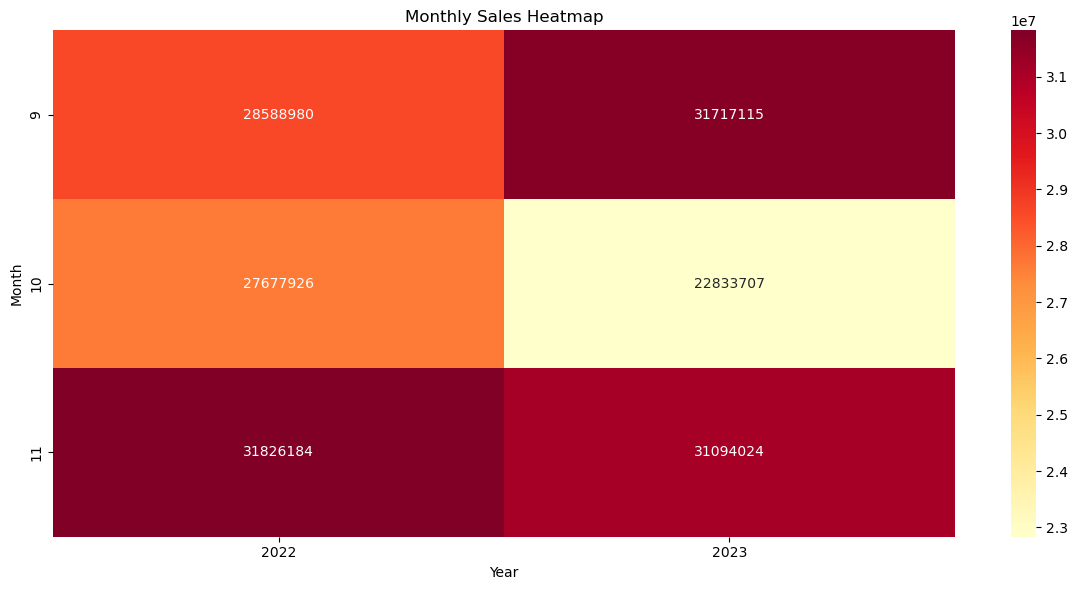
\includegraphics[width=1\columnwidth]{images/month.png}
        \end{center}
    }
    \item Also we can see find month by month over year sales.{
        \begin{center}
            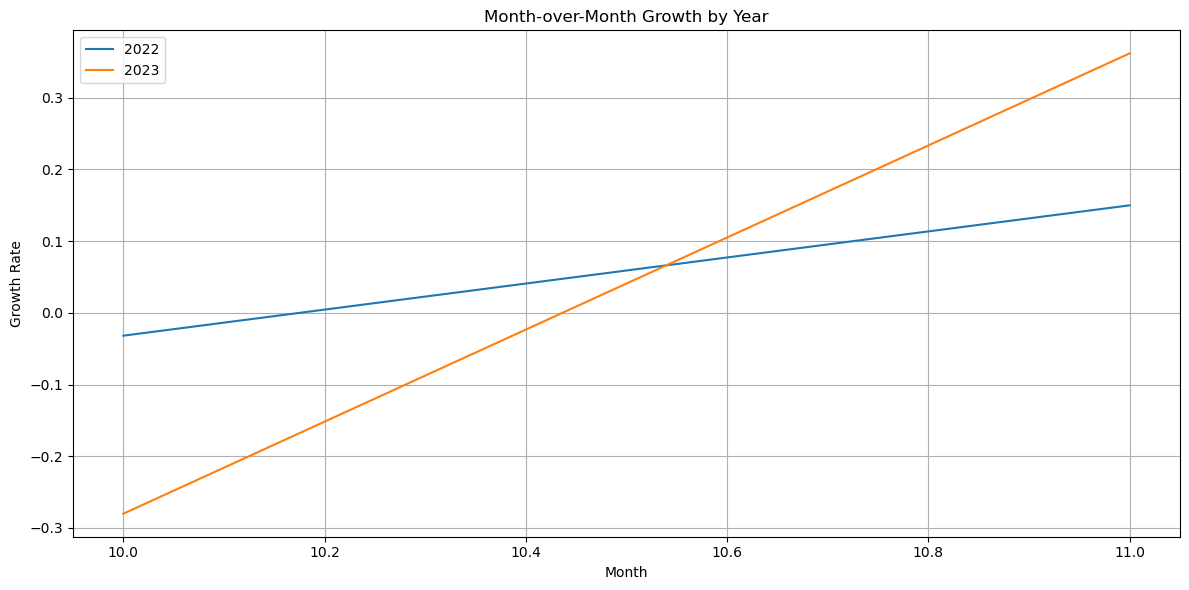
\includegraphics[width=1\columnwidth]{images/month-growth.png}
        \end{center}
    }
\end{itemize}

    \subsection{Average Order Value (AOV)}
    \begin{itemize}
        \item Analyze trends in average order value over time.{
            \begin{center}
                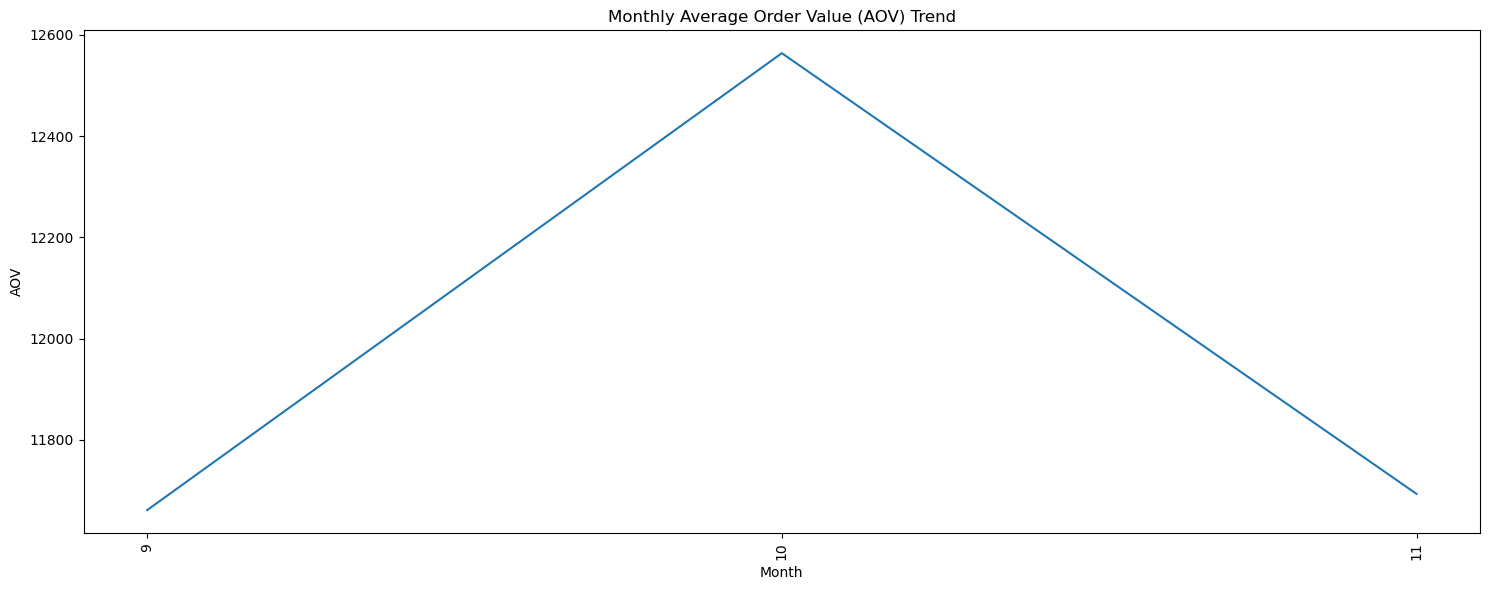
\includegraphics[width=1\columnwidth]{images/month-aov.png}
            \end{center}
            \textbf{Insights:}
            \begin{itemize}
                \item The aov is clearly showing an increase in sales upto october and then a decrease from there.
                \item It means months aroung October has higher sales and demand than other months beacuse of festivals season.
            \end{itemize}
        }
    \end{itemize}


\section{4. SKU Performance Analysis}
    \subsection{Top-Selling SKUs}
    \textbf{First lets see which are SKUs that are top selling.}
    \begin{center}
        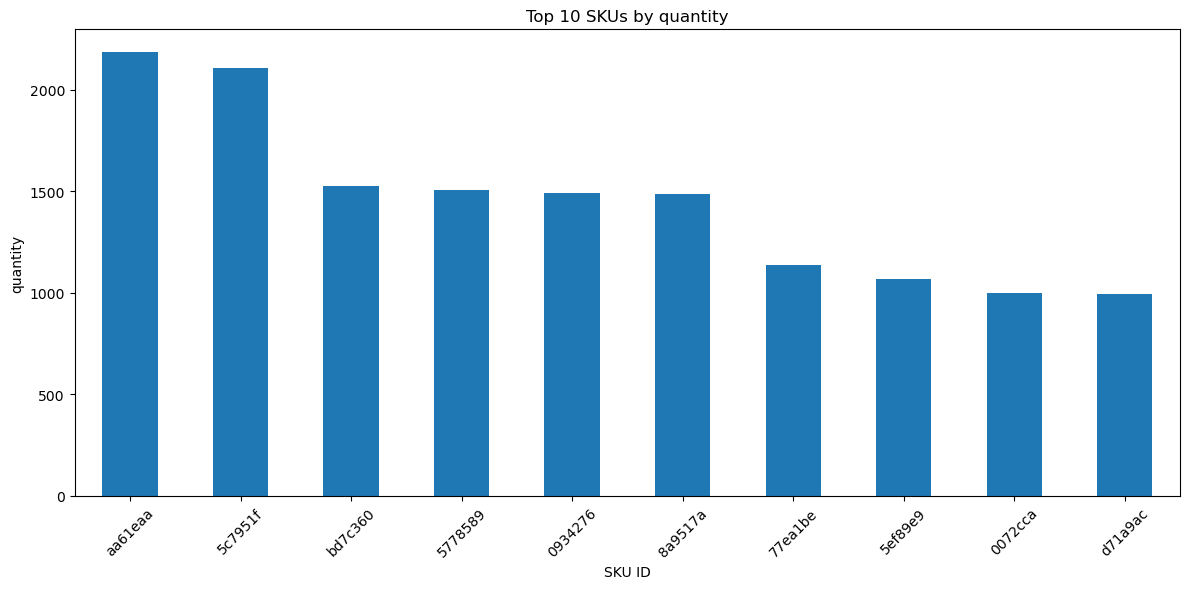
\includegraphics[width=1\columnwidth]{images/top-skus.png}
    \end{center}
    \caption{Top 10 Selling SKUs by Quantity.}
    \vspace{0.2in}
    Also lets see the top selling SKUs by GMV.{
       \begin{verbatim}
Top 10 SKUs by placed_gmv:

sku_id
aa61eaa    3358729.54
bd7c360    3033729.76
5778589    2004186.77
0072cca    1818349.65
8a9517a    1770669.35
0934276    1691484.70
5c7951f    1674269.10
ee90f3e    1285239.63
be170aa    1270098.64
6323dad    1269127.86
Name: placed_gmv, dtype: float64
       \end{verbatim}
    }
    
    \subsection{SKU Diversity}
    
    \texttbf{Analyze the diversity of SKUs in customer orders.}
    \large
    What this means is that how many unique SKUS are their in any order_ID.
    \normalsize
    \begin{center}
        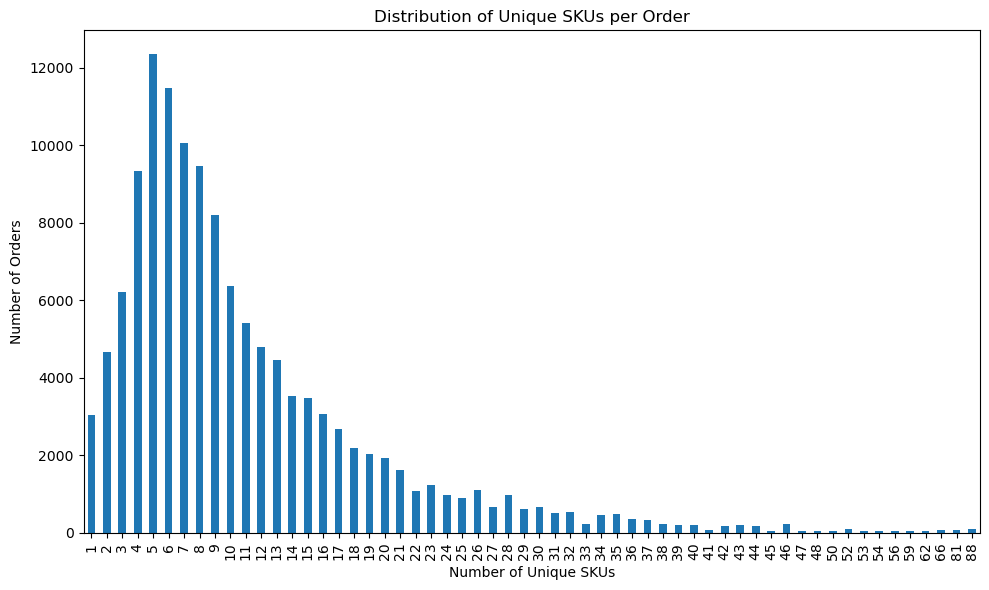
\includegraphics[width=1\columnwidth]{images/sku-dis.png}
    \end{center}
    \begin{tcolorbox}[colback=lightPink!5!white,colframe=lightPink!75!black,title=Insights]
        \textbf{Insights:}
        \begin{itemize}
            \item Majority of the orders contain 1-14 unique SKUs, meaning customers tend to buy a variety of products in a single order.
            \item But customers buying more than 14-15 unique SKUs are very less.
            \item 7 is the most common number of unique SKUs in an order.
        \end{itemize}
    \end{tcolorbox}
  
    

    \subsection{ABC Analysis}
    \textbf{Perform ABC analysis to categorize SKUs based on sales contribution.}
    \begin{itemize}
        \item   Category A SKUs (up to 80\% of GMV) are the most critical for driving sales and revenue.
        \item Category B SKUs contribute moderately (the next 15\% of GMV).
        \item Category C SKUs (final 5\%) are the least significant for overall revenue.
    \end{itemize}
    \begin{center}
        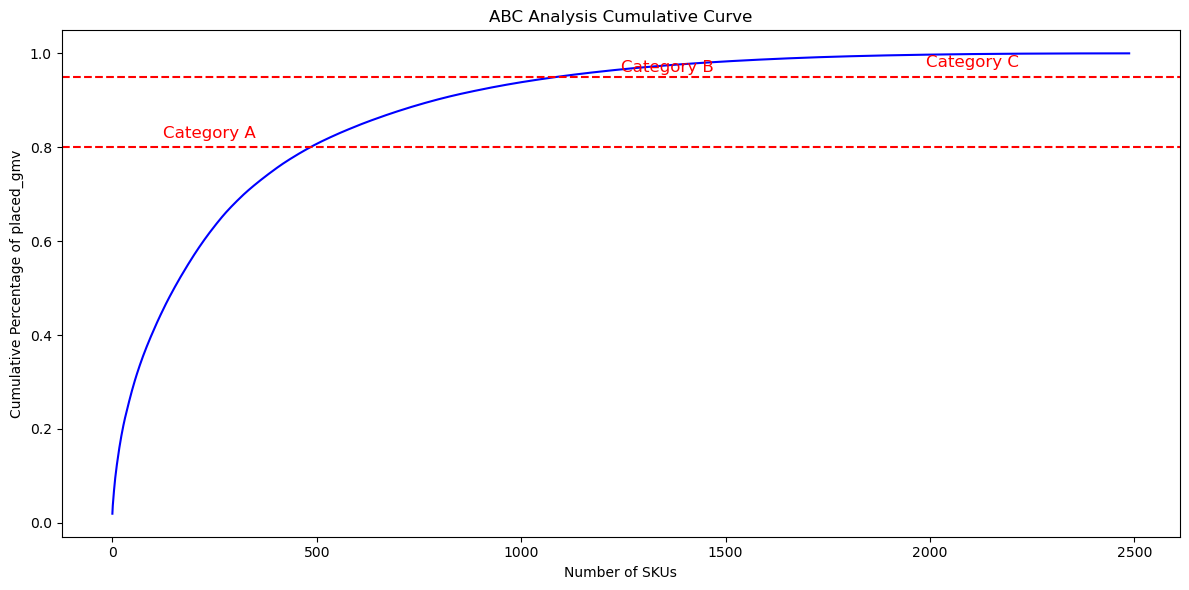
\includegraphics[width=1\columnwidth]{images/abc.png}
    \end{center}
One key observations that can be noticed is that \textbf{Only less than 500 unique SKU's are contributing to 80\% of the GMV.}
\textbf{Extensive results is as follows:}
\begin{verbatim}
    ABC Analysis Results:
    placed_gmv
    A     484
    B     605
    C    1398
    Name: count, dtype: int64
    
    Percentage of SKUs in each category:
    placed_gmv
    A    19.453376
    B    24.316720
    C    56.189711
    Name: count, dtype: float64
\end{verbatim}


    
    \subsection{Purchase Patterns}
    \textbf{Purchase patterns for top-selling SKUs.}
    \begin{center}
        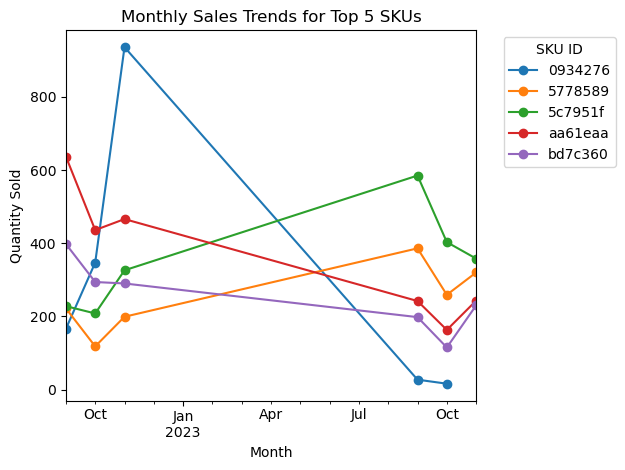
\includegraphics[width=1\columnwidth]{images/month-sku.png}
    \end{center}
    \caption{As already seen, the top selling SKUs are sold more in the month of October and November.}

    \subsection{Correlated SKU Pairs:}
    \textbf{Correlated SKU pairs that are frequently purchased together.}
    \begin{center}
        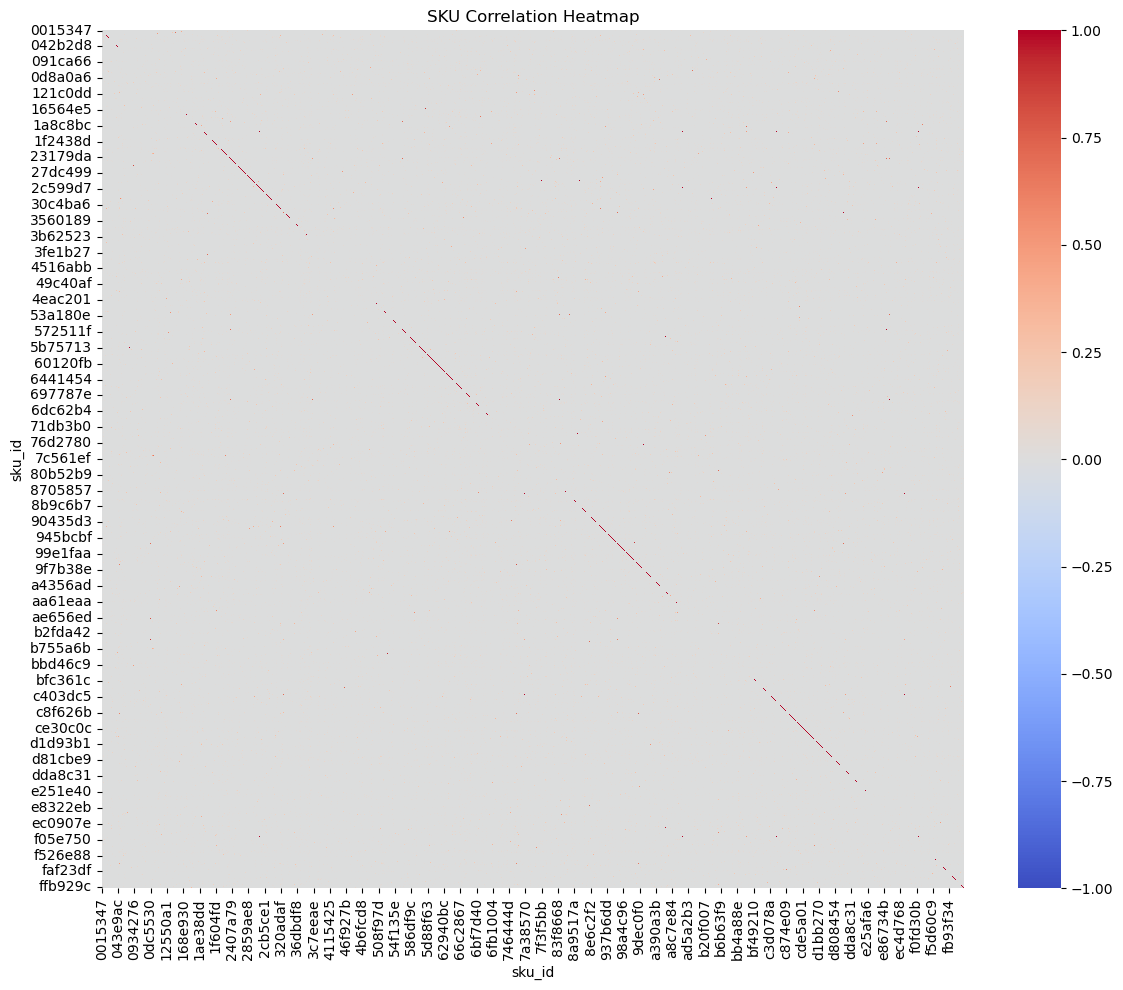
\includegraphics[width=1\columnwidth]{images/corr-sku.png}
    \end{center}
    \begin{verbatim}
 Top 10 Correlated SKU Pairs:

sku_id   sku_id     sku_corr
320adaf  a6ae1cb    0.991596      
a6ae1cb  320adaf    0.991596
320adaf  581e5e8    0.991561
581e5e8  320adaf    0.991561
         a6ae1cb    0.987324
a6ae1cb  581e5e8    0.987324
a2633d6  af6266b    0.979263
af6266b  a2633d6    0.979263
320adaf  ed18f1c    0.962180
ed18f1c  320adaf    0.962180
    \end{verbatim}


\section{5. Order Analysis}
    \subsection{Order Sizes}
    \begin{center}
       
            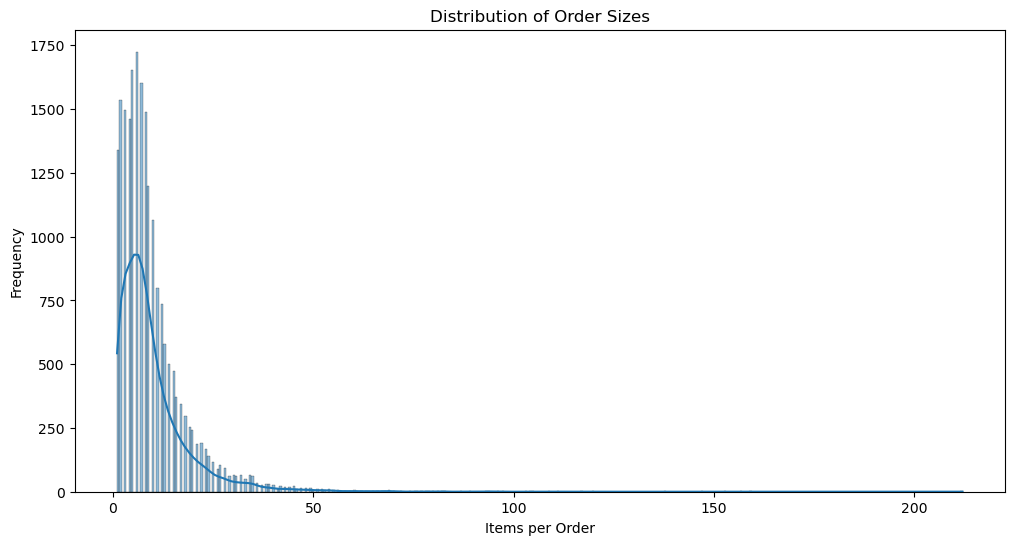
\includegraphics[width=1\columnwidth]{images/order-size.png}
      
    \end{center}
    \textbf{Insights: Majority of the items per order is less than 30 only,\\
     indicating that most customers tend to buy a small number of items in a single order.}
    
    \subsection{Relationship Between Order Size and GMV}
    \begin{center}
        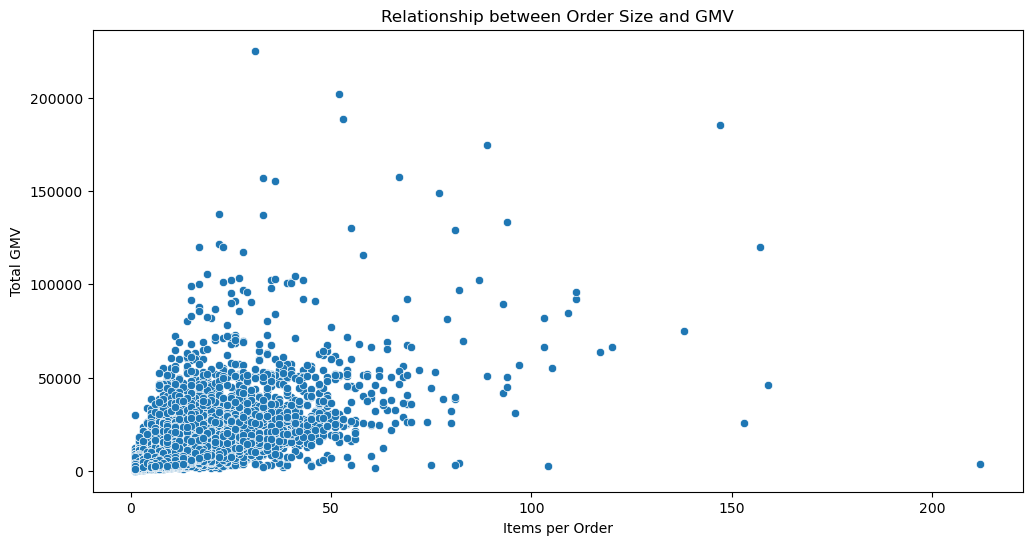
\includegraphics[width=1\columnwidth]{images/order-gmv.png}
    \end{center}
    \begin{verbatim}
Average GMV by order size:
    items_per_order      total_gmv
0               1.0    3376.119590
1               2.0    3969.668248
2               3.0    4018.977017
3               4.0    4210.006826
4               5.0    5036.383487
..              ...            ...
95            147.0  185110.060000
96            153.0   25552.700000
97            157.0  119976.360000
98            159.0   46079.400000
99            212.0    3579.440000

    \end{verbatim}
    
    \subsection{Multi-item Orders}
    \begin{verbatim}
Comparison of single-item vs multi-item orders:
                   avg_gmv  order_count
is_multi_item                          
False          3376.119590         1340
True           8546.590083        19799

From this we can see that multi-item orders have higher average GMV than single-item orders and also have more order count.
Seasonal patterns in orders:
   month   quantity   placed_gmv
0      9   9.416080  7858.495579
1     10  10.319842  8699.902473
2     11   9.747356  8215.198914
    \end{verbatim}
    \begin{center}
        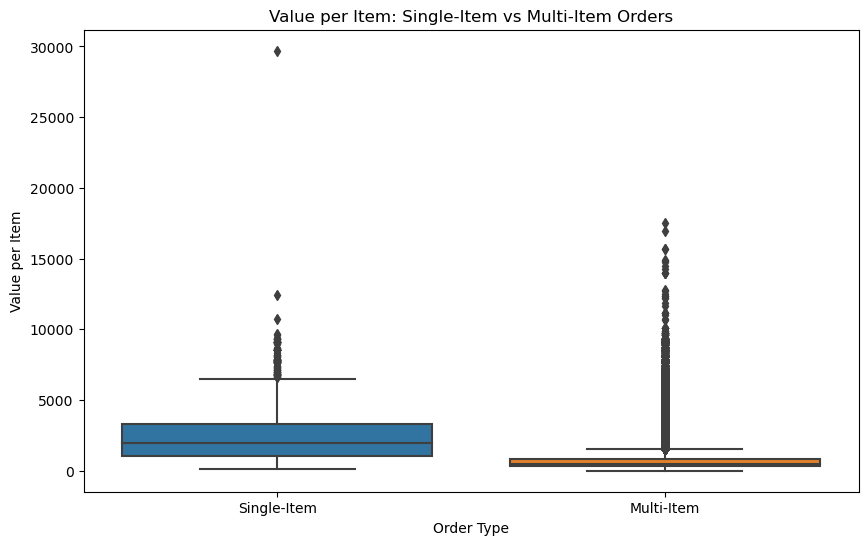
\includegraphics[width=1\columnwidth]{images/value-per.png}
    \end{center}
    \textbf{Insights: If a customer is buying more items in a single order,\\
     then the value per item is low, meaning they are buying cheaper items if buying multiple items.\\
     But if they are buying single item, then the value of that item is high.}

\section{6. Cohort Analysis}
    \subsection{Customer Cohorts}
    \begin{itemize}
        \item Create cohorts based on the first purchase date of customers.
    \end{itemize}
    
    \subsection{Cohort Retention}
    \begin{center}
        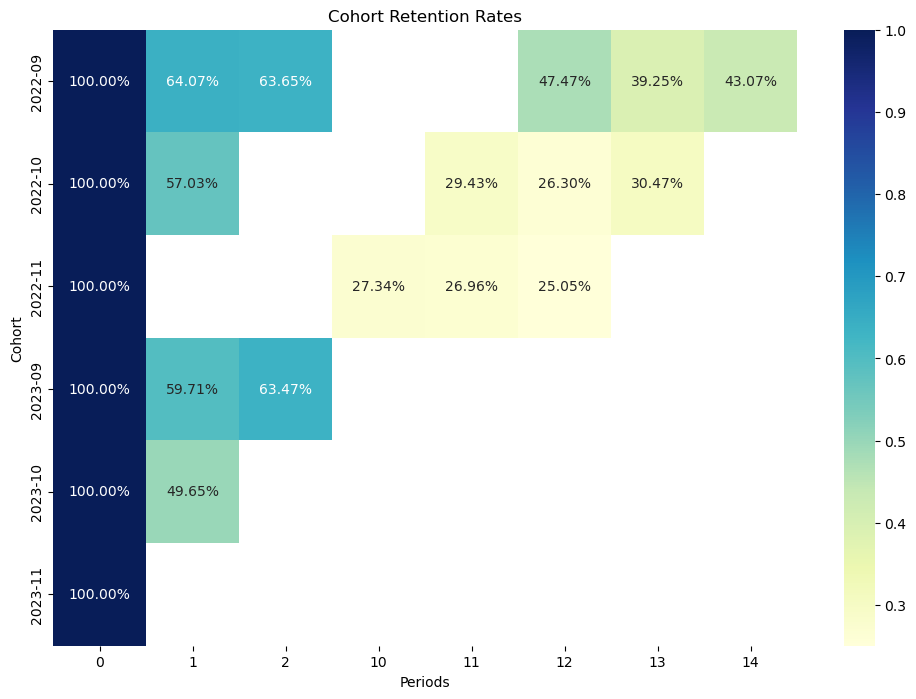
\includegraphics[width=1\columnwidth]{images/cohort-retention.png}
    \end{center}
    \begin{itemize}
        \item \textbf{High Initial Retention:} All cohorts begin with a 100\% retention rate, as expected at the start of the analysis period.
        
        \item \textbf{Declining Retention:} Retention rates drop consistently over time for all cohorts, showing typical user drop-off after acquisition.
        
        \item \textbf{Best Performance by 2022-09 Cohort:} The 2022-09 cohort maintains relatively high retention rates across longer periods, with 47.47\% after Period 4 and 43.07\% after Period 6.
        
        \item \textbf{Improved Retention for Recent Cohorts:} The 2023-09 and 2023-10 cohorts show improved retention compared to earlier cohorts, with the 2023-09 cohort peaking at 63.47\% in Period 2.
        
        \item \textbf{Sharp Decline for 2022-10 Cohort:} The 2022-10 cohort experiences a sharp drop from 100\% to 57.03\% after the first period and continues to decline significantly afterward.
        
        \item \textbf{Retention Stabilization:} Some cohorts, like the 2022-09, show retention stabilization around 30-40\% over extended periods.
    \end{itemize}
    

\section{7. Geographic Analysis}
    \begin{itemize}
        \item Which of the Region has highest average sales.{
             \begin{center}
                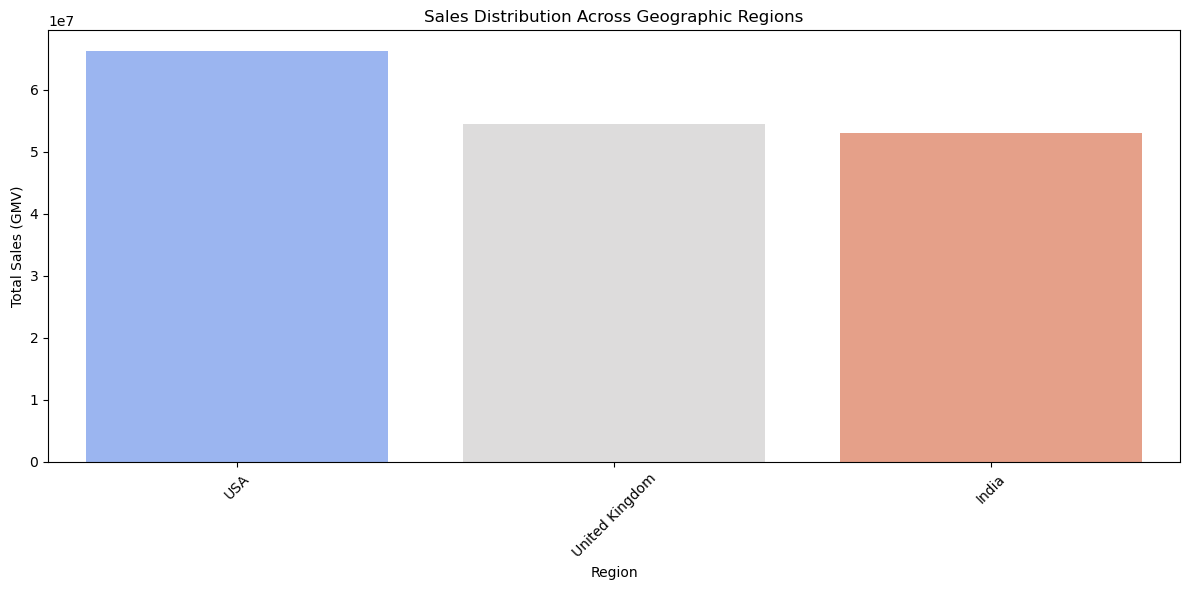
\includegraphics[width=1\columnwidth]{images/region.png}
             \end{center}
             \textbf{Insights: From the plot, USA has the highest average sales while India has lowest.}
        }
        \item Identify high-performing and underperforming areas.{
            \begin{verbatim}
High-performing areas by region:
warehouse_name
USA    66248696.45

Underperforming areas:
warehouse_name
United Kingdom    54423087.40
India             53066153.46
            \end{verbatim}
   
        }
    \end{itemize}

    
    \subsection{Promotion Opportunities}
    \textbf{On which days, promotions should be given to increase sales.}
    \begin{verbatim}
Days of the week with below-average sales:
day_of_week
2              19264706.77
3              19741434.06
5              22500186.65
6              17285881.25
    \end{verbatim}



\section{8. Customer Lifetime Value (CLV) Analysis}

    \subsection{CLV Calculation}
    \begin{itemize}
        \item CLV is calculated by multiplying the total revenue generated by a customer with their estimated lifespan, assuming yearly CLV.
        \item Metrics such as total revenue, average order value (AOV), purchase frequency, and customer lifespan are included in the calculation.
    \end{itemize}
    
    \subsection{CLV Influencing Factors}
    \begin{center}
        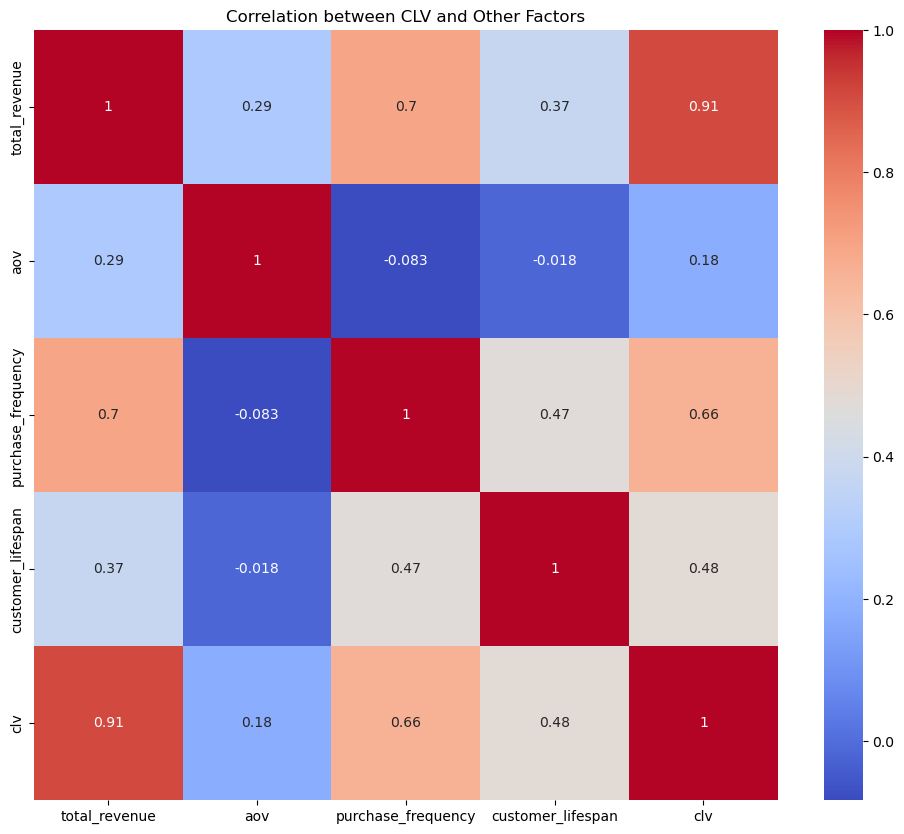
\includegraphics[width=1\columnwidth]{images/clf-factor.png}
    \end{center}
    \begin{itemize}
        \item \textbf{Total Revenue:} Strong positive correlation with CLV (0.91). Customers generating higher revenue have significantly higher CLV.
        \item \textbf{Purchase Frequency:} Moderate positive correlation with CLV (0.66). Frequent buyers tend to have higher CLV.
        \item \textbf{Customer Lifespan:} Weak to moderate positive correlation with CLV (0.48). The longer a customer stays active, the higher their CLV, but this impact is smaller compared to revenue and frequency.
        \item \textbf{Average Order Value (AOV):} Weak positive correlation with CLV (0.18). AOV has a relatively small impact, indicating that frequent purchases are more important than high-value purchases.
    \end{itemize}
    
    \subsection{Insights on revenue, AOV, and purchase frequency}
    \begin{itemize}
        \item \textbf{Total Revenue and Purchase Frequency:} Strong positive correlation (0.70). Customers who purchase more frequently tend to generate higher total revenue.
        \item \textbf{AOV and Purchase Frequency:} Slight negative correlation (-0.083). Customers making larger purchases tend to buy less frequently, suggesting a trade-off between order size and frequency.
    \end{itemize}
    
    \subsection{Customer Segmentation Based on CLV}
    \begin{itemize}
        \item \textbf{High-Value Customers:} Identified as those in the top 25\% of CLV. These customers contribute a significant portion of revenue and tend to have higher purchase frequency.
        \item \textbf{Low-Value Customers:} Identified as those in the bottom 25\% of CLV. These customers have lower revenue, fewer purchases, and shorter lifespans.
    \end{itemize}
    
    \subsection{CLV Distribution}
    \begin{itemize}
        \item The distribution of CLV shows a skewed pattern, with a smaller number of high-value customers contributing a disproportionate amount of revenue, while a larger segment consists of low-value customers.
    \end{itemize}

\section{9. Basket Analysis}
    \subsection{Market Basket Analysis}
    In this section, I will find which pairs are most likely to bought together.
    \begin{verbatim}
Most freq. product combinations in multi-item orders:            Count  SKU_ID 
(aa61eaa, bd7c360)                                               183    12
(0eeddec, 8705857)                                               159    11
(d0990b0, f4575a8)                                               143     8
(941d30b, cb91396)                                               137     8
(92e3cb7, d0990b0)                                               115     6
(8ae2033, 92e3cb7)                                               114     6
(0eeddec, 77ea1be)                                               110     6
(0934276, 56f9240)                                               104     6
(380b808, 5ef89e9)                                               103     5
(0085272, 385c311)                                                98     5

    \end{verbatim}

\section{10. Price Sensitivity Analysis}
    \subsection{Price vs. Demand}
    \begin{center}
        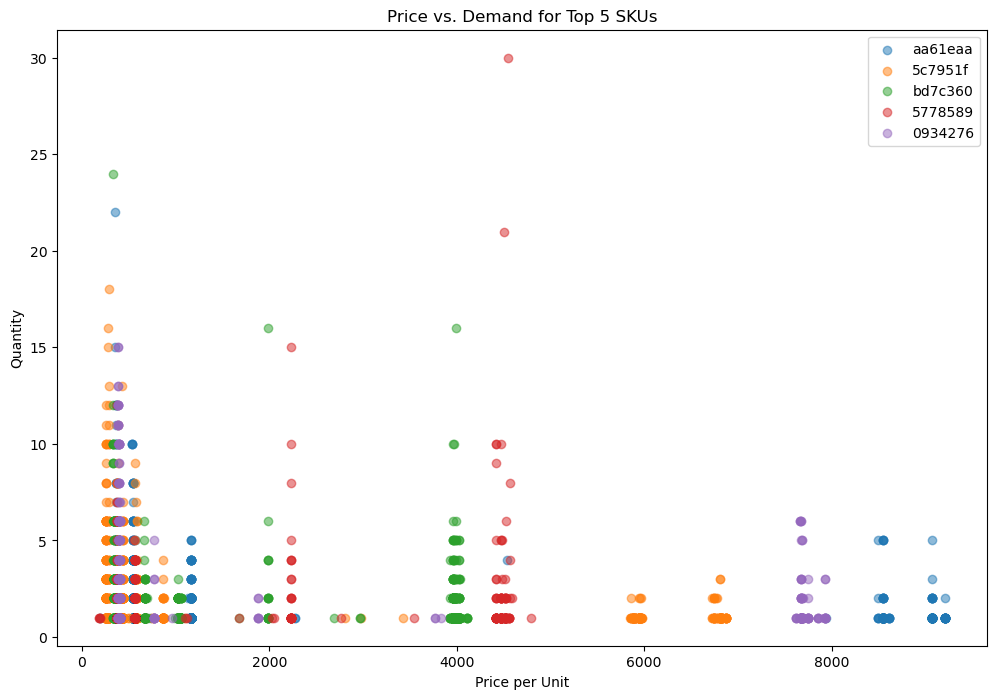
\includegraphics[width=1\columnwidth]{images/price-demand.png}
    \end{center}
    \begin{itemize}
        \item The demand for SKUs is generally higher at lower prices, as seen by the dense clustering of points on the left side of the plot, where the price per unit is less than 2000.
        \item The SKU labeled '0934276' (purple) shows a broad distribution of prices, ranging from very low to as high as 8000, with a consistent but low quantity sold across this range.
        \item The SKU labeled 'aa61eaa' (blue) demonstrates significant demand even at higher prices, peaking around 8000, suggesting a premium product with stable demand.
        \item There's a notable drop in demand as the price increases beyond 2000 for most SKUs, indicating price sensitivity among customers for these products.
        \item Most of the data points for all SKUs are concentrated around quantities less than 10, indicating that bulk purchases are less common, regardless of price.
        \item The SKU '5778589' (red) has instances of high demand (quantities around 15-20) at lower price points, suggesting it is a popular choice when priced competitively.
    \end{itemize}
    

    \newpage

\vfill

\begin{center}
    \color{red}\rule{1\linewidth}{1mm}
    % write thank You
    \vspace{4in}

    \Huge\textbf{Thank You}
\end{center}
\vfill


\end{document}